\documentclass[12pt, twoside]{article}
%\documentclass[12pt, twoside]{article}
\usepackage[letterpaper, margin=1in, headsep=0.2in]{geometry}
\setlength{\headheight}{0.6in}
%\usepackage[english]{babel}
\usepackage[utf8]{inputenc}
\usepackage{microtype}
\usepackage{amsmath}
\usepackage{amssymb}
%\usepackage{amsfonts}
\usepackage[nomessages]{fp} %\FPeval{\var-name}{2*sin(pi/6)}
\usepackage{siunitx} %units in math. eg 20\milli\meter
\usepackage{yhmath} % for arcs, overparenth command
\usepackage{tikz} %graphics
\usetikzlibrary{quotes, angles, arrows, arrows.meta}
\usepackage{pgfplots}
\usepgfplotslibrary{fillbetween}
\pgfplotsset{compat=1.16}
\usepackage{graphicx} %consider setting \graphicspath{{images/}}
\usepackage{parskip} %no paragraph indent
\usepackage{enumitem}
\usepackage{multicol}
\usepackage{venndiagram}

\usepackage{fancyhdr}
\pagestyle{fancy}
\fancyhf{}
\renewcommand{\headrulewidth}{0pt} % disable the underline of the header
\raggedbottom
\hfuzz=2mm %suppresses overfull box warnings

\usepackage{hyperref}

\fancyhead[LO]{La Scuola d'Italia / Dr.\ Huson / IB Math 11 \\* 2 November 2026}
\fancyhead[RO]{\fbox{\begin{minipage}{6cm}\footnotesize Nickname:\\[0.5cm]\end{minipage}}}
\fancyfoot[C]{\thepage}

\begin{document}
\subsubsection*{2.7 Challenge: Systems of Equations and Market Equilibrium (no calculator)}

\begin{enumerate}[itemsep=0.15cm]

%--- Problem 1: Supply and demand lines; estimate equilibrium from graph; solve by elimination; interpret gradient; price ceiling shortage; consumer surplus triangle [13 marks] ---
%--- Source: Original (AA SL 2.1, systems of linear equations, 3.1 area); market context ---
\item[1.]

\begin{minipage}[t]{0.45\textwidth}
The market for phone cases in a city is modelled by two straight lines.
The quantity is $q$ thousand cases per month and the price is $p$ euros
per case.

\medskip
Demand line $D$: \quad $p = 50 - 3q$

\smallskip
Supply line $S$: \quad $p = 10 + 2q$

\medskip
The market is in \emph{equilibrium} at the point where the two lines
intersect.
\end{minipage}
\hfill
\begin{minipage}[t]{0.48\textwidth}
\vspace{0pt}
\begin{tikzpicture}
\begin{axis}[
  axis lines=left,
  xlabel={$q$}, ylabel={$p$},
  xlabel style={at={(axis description cs:1,0)}, anchor=north west},
  ylabel style={at={(axis description cs:0,1)}, anchor=south east, rotate=-90},
  xmin=0, xmax=18, ymin=0, ymax=55,
  xtick={0,2,...,16}, ytick={0,10,...,50},
  grid=major, grid style={line width=0.2pt, gray!40},
  tick label style={font=\footnotesize},
  width=7.6cm, height=6cm,
]
  \addplot[very thick, domain=0:16.2] {50 - 3*x};
  \addplot[very thick, dashed, domain=0:16] {10 + 2*x};
  \node[fill=white, inner sep=1pt, font=\small] at (axis cs:15.6,12) {$D$};
  \node[fill=white, inner sep=1pt, font=\small] at (axis cs:16.6,47) {$S$};
\end{axis}
\end{tikzpicture}
\end{minipage}

\begin{enumerate}[itemsep=0.1cm]
  \item Use the graph to estimate the equilibrium quantity and price.
  \item Write both equations in the form $aq + bp = c$. Hence, use the
  elimination method to find the exact equilibrium quantity and price.
  \item Write down the gradient of the supply line. Interpret this value
  in context.
  \item The city sets a maximum price of $20$ euros per case. Find the
  quantity demanded and the quantity supplied at this price. Hence, find
  the shortage of phone cases.
  \item The \emph{consumer surplus} is the area of the triangle between the
  demand line, the $p$-axis and the horizontal line at the equilibrium
  price. Shade this triangle on the graph and find the consumer surplus
  in euros.
\end{enumerate}

\begin{tikzpicture}
  \draw (-0.6,0) rectangle (14.6,8.6);
  \foreach \y in {1,2,...,8} \draw[dotted] (0,\y)--(14.1,\y);
\end{tikzpicture}

\newpage

%--- Problem 2: Two-account investment, set up and solve 2x2 by elimination with scaling; extension three-fund 3x3 system [11 marks] ---
%--- Source: Original (AA SL 2.1 systems, 1.4 simple interest context); extension part (c) for the advanced group ---
\item[2.]

Giulia invests $10\,000$ euros for one year. She puts $x$ euros into a
savings bond that pays $3\%$ interest per year and the remaining $y$ euros
into a fund that pays $7\%$ per year. After one year she has earned $540$
euros in interest.

\begin{enumerate}[itemsep=0.1cm]
  \item Write down two equations in $x$ and $y$.
  \item Use the elimination method to find the amount invested in the
  bond and the amount invested in the fund.
\end{enumerate}

\textbf{Extension.} Marco invests $20\,000$ euros for one year in three
funds. He puts $x$ euros into a fund paying $2\%$ per year, $y$ euros
into a fund paying $4\%$ and $z$ euros into a fund paying $6\%$. He earns
$740$ euros in interest. He puts $2000$ euros more into the $4\%$ fund
than into the $6\%$ fund.

\begin{enumerate}[itemsep=0.1cm]
  \item[(c)] \begin{enumerate}[label=(\roman*), itemsep=0.1cm]
    \item Write down three equations in $x$, $y$ and $z$.
    \item Use the elimination method to find $x$, $y$ and $z$.
  \end{enumerate}
\end{enumerate}

\begin{tikzpicture}
  \draw (-0.6,0) rectangle (14.6,14.4);
  \foreach \y in {1,2,...,14} \draw[dotted] (0,\y)--(14.1,\y);
\end{tikzpicture}

\end{enumerate}
\end{document}
